% circuit-sim-lab-report — report.tex
% Course 0714-EEE-2102, Circuit Simulation Laboratory
% Experiment 4 — full-wave bridge rectifier with and without filter capacitor
%
% Compile (twice, from Lab_report_latex/):
%   env pdflatex -interaction=nonstopmode report.tex

\documentclass[12pt,a4paper]{article}

% ----- Page geometry: A4, 1 inch margins all sides -----
\usepackage[margin=1in]{geometry}

% ----- Times New Roman (text + math) -----
\usepackage{newtxtext,newtxmath}

% ----- Spacing: 1.5 line spacing, 6 pt paragraph spacing -----
\usepackage{setspace}
\onehalfspacing
\usepackage{parskip}          % paragraph gaps instead of indents
\setlength{\parskip}{6pt plus 1pt}

% ----- Math, SI units -----
\usepackage{amsmath}
\usepackage{siunitx}

% ----- Graphics, tables, captions, floats -----
\usepackage{graphicx}
\usepackage{booktabs}
\usepackage[american]{circuitikz}
\usepackage{caption}
\usepackage{float}
\usepackage{array}
\usepackage[table]{xcolor} % row shading for Word-style table headers
\graphicspath{{../graphs/}{./figures/}}

% ----- Lists: compact, guide-style itemization -----
\usepackage{enumitem}
\setlist{nosep, leftmargin=2em, label=\textbullet}

% ----- Front matter and PDF output -----
\usepackage{pdfpages}
\usepackage[hidelinks]{hyperref}

% ----- Headings: bold, left-aligned, 14/15 pt -----
\usepackage{titlesec}
\titleformat{\section}
{\normalfont\Large\bfseries}{\thesection}{0.8em}{}
\titleformat{\subsection}
{\normalfont\large\bfseries}{\thesubsection}{0.8em}{}
\titlespacing*{\section}{0pt}{*3}{*2}
\titlespacing*{\subsection}{0pt}{*2.5}{*1.5}

% ----- Captions: centered, 11 pt, figures below / tables above -----
\captionsetup{font=small, labelfont=bf, justification=centering}
\captionsetup[table]{position=above, skip=4pt, labelfont=normalfont}
\captionsetup[figure]{position=below, skip=4pt, labelfont=normalfont}

% ----- Page number: bottom-center -----
\usepackage{fancyhdr}
\pagestyle{fancy}
\fancyhf{}
\fancyfoot[C]{\thepage}
\renewcommand{\headrulewidth}{0pt}

% ----- Experiment number: sections then number 4.1-4.9 -----
\newcommand{\expnumber}{4}
\renewcommand{\thesection}{\expnumber.\arabic{section}}

\begin{document}
	
	% =====================================================================
	% FRONT MATTER (pages 1-2): cover page and task sheet
	% =====================================================================
	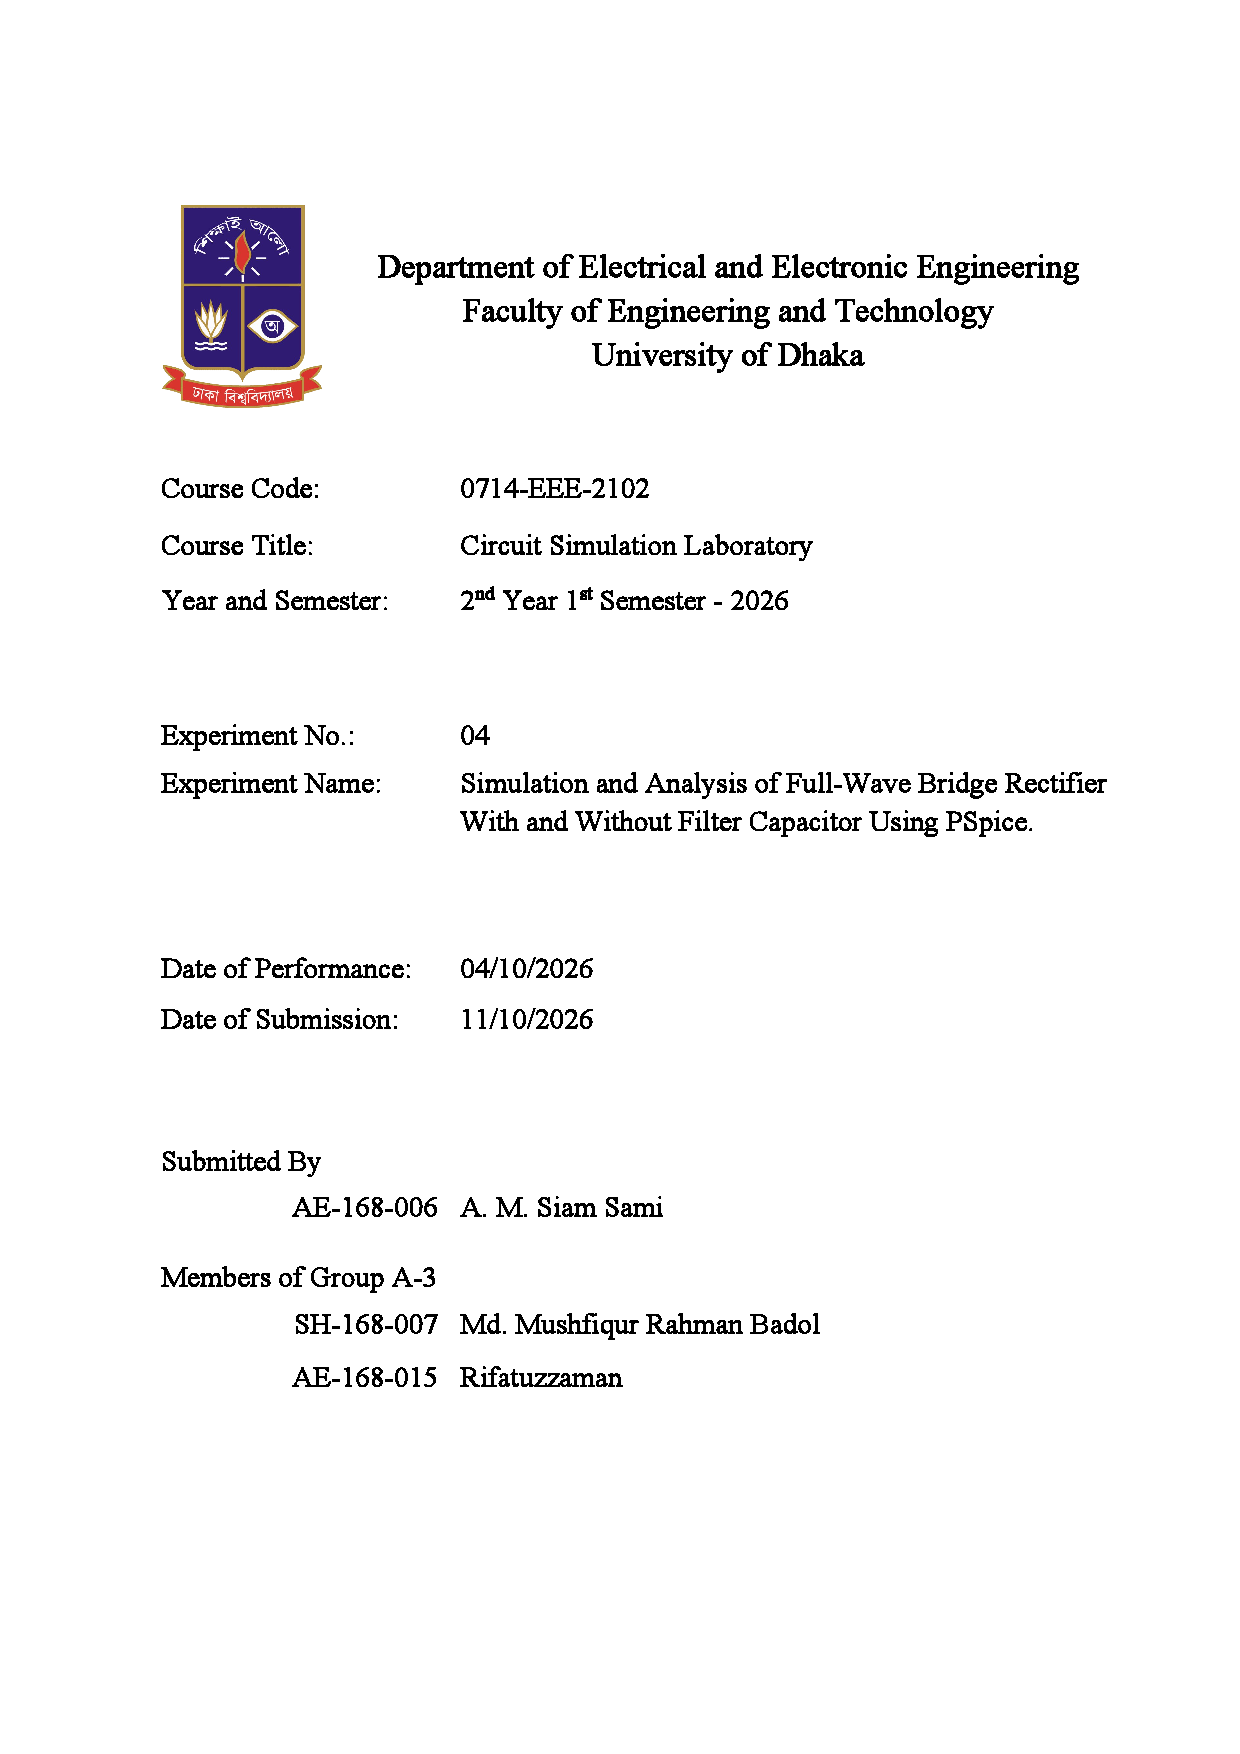
\includepdf[pages={1}]{../Cover_page.pdf}
	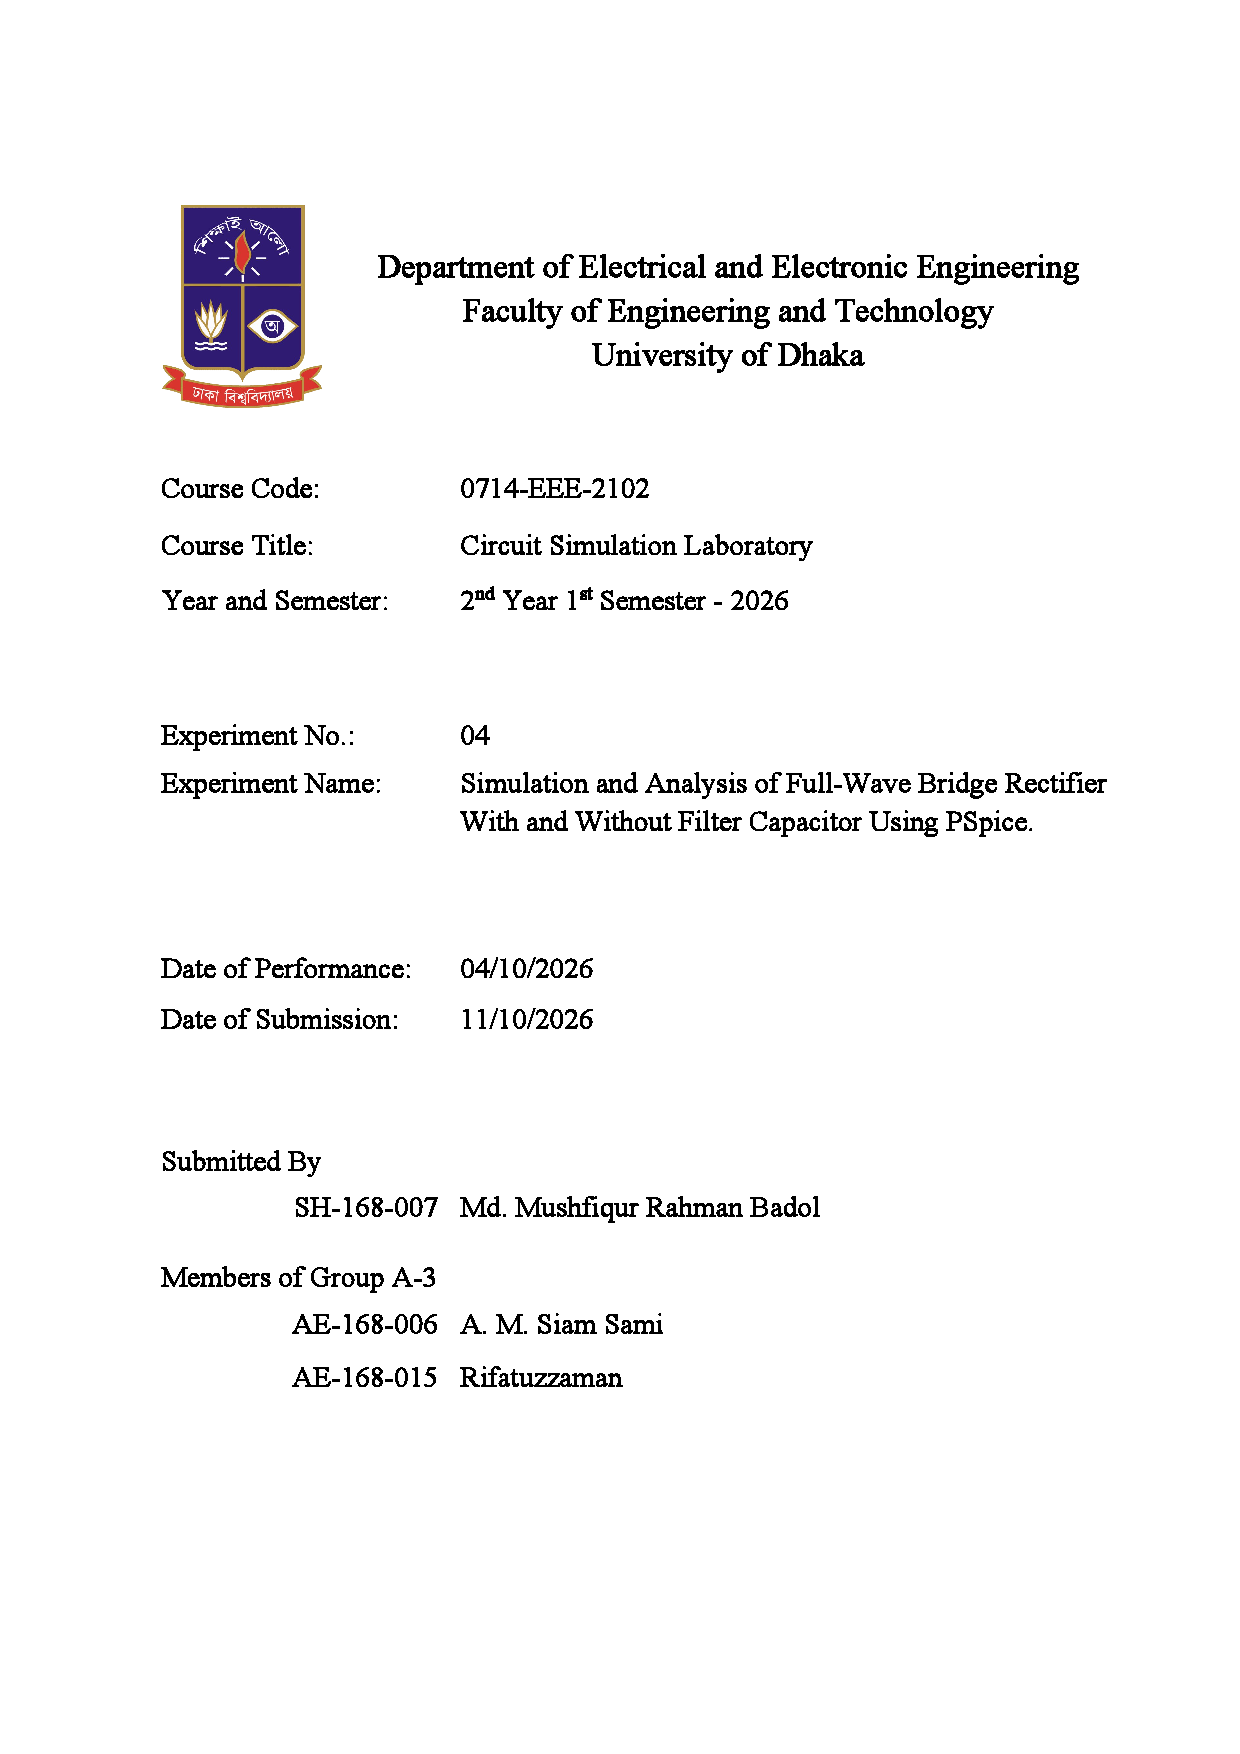
\includepdf{../Cover_badol.pdf}
	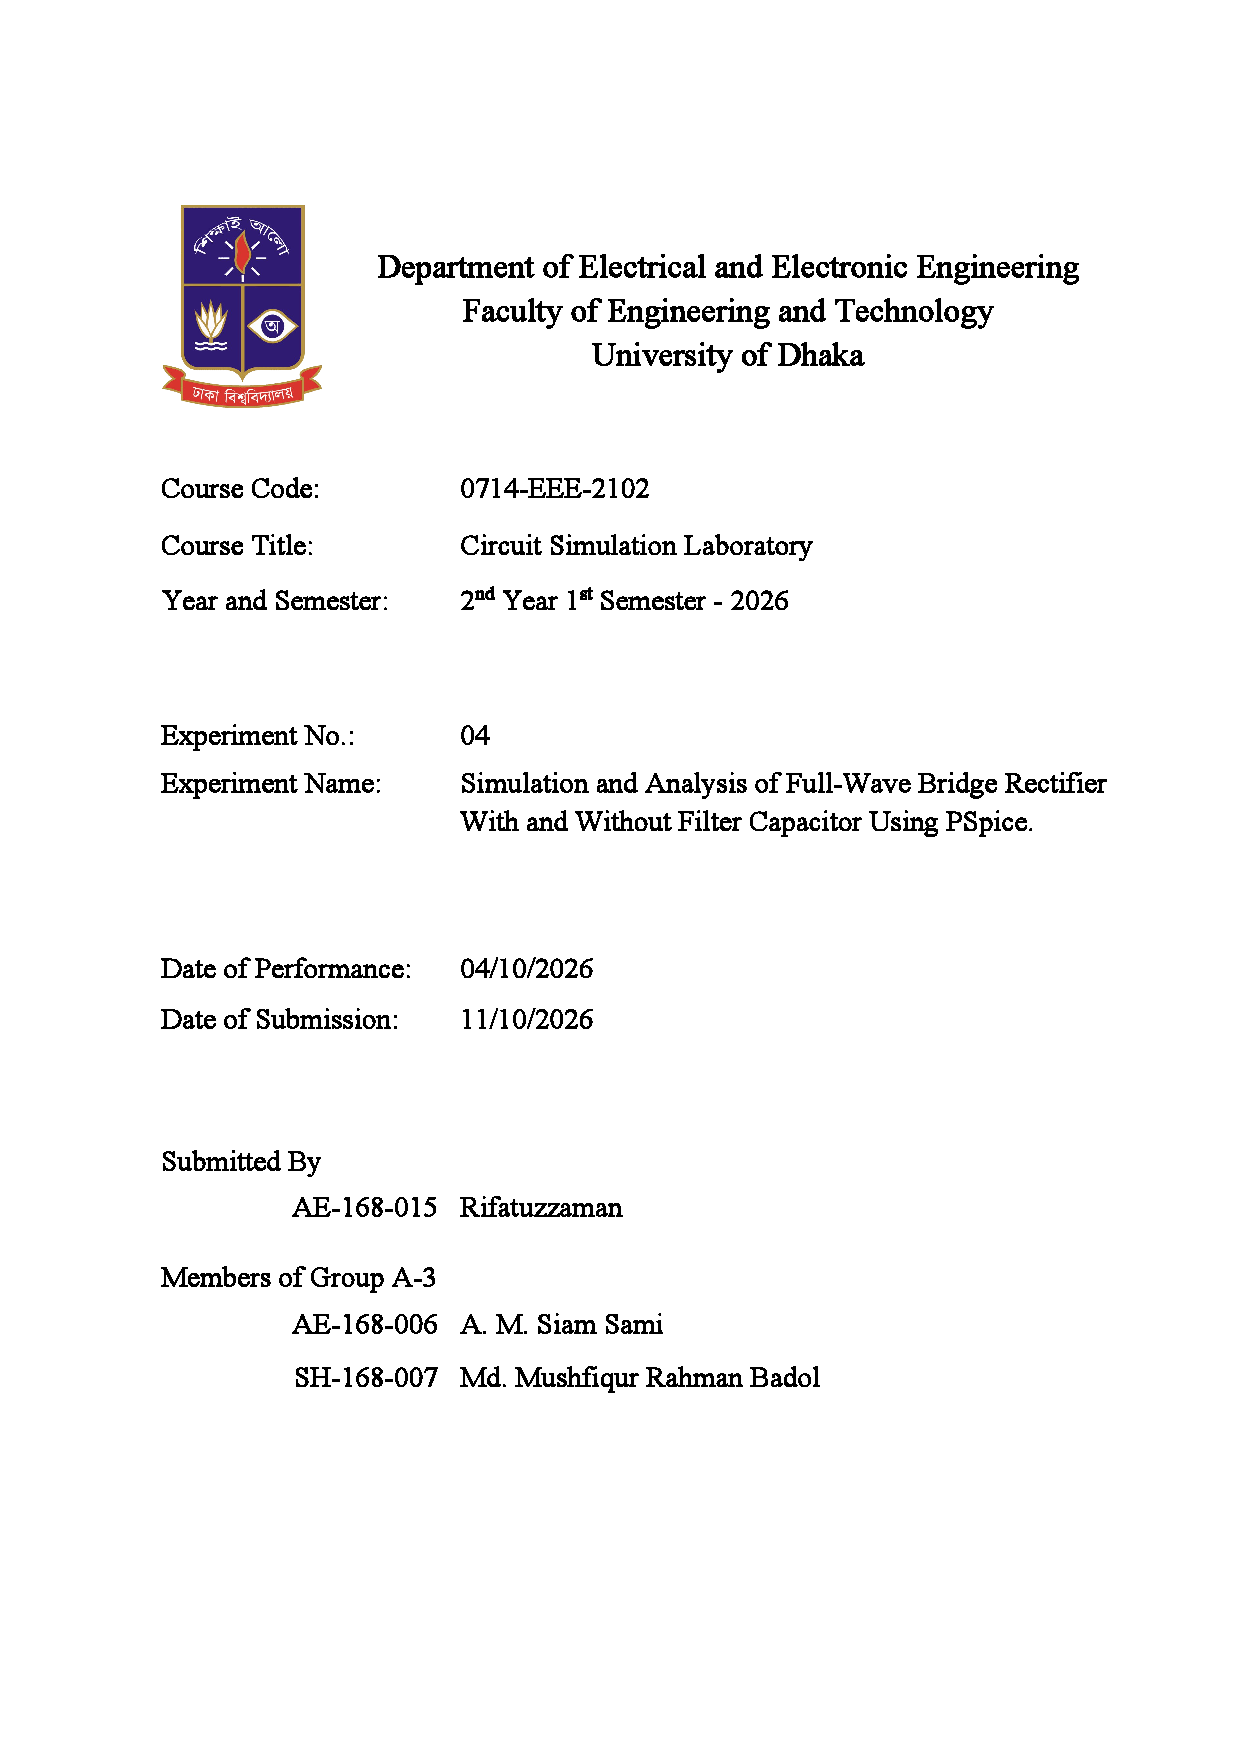
\includepdf{../Cover_rifatuzzaman.pdf}
	
\includepdf[pages={1}]{../2nd_page.pdf}
	% =====================================================================
	% HEADER BLOCK
	% =====================================================================
	\begin{center}
		{\large\bfseries Experiment No. \expnumber}\\[4pt]
		{\large\bfseries Name of the Experiment: Simulation and Analysis of
			Full-Wave Bridge Rectifier With and Without Filter Capacitor
			Using PSpice}
	\end{center}
	\vspace{6pt}
	
	% =====================================================================
	\section{Objective}
	% =====================================================================
	The purposes of this experiment are-
	\begin{enumerate}[label=\arabic*.]
		\item Designing and simulating a full-wave bridge rectifier without a filter capacitor in PSpice and determining its input and output waveforms.
		\item Designing and simulating the full-wave bridge rectifier with a filter capacitor and analyzing the capacitor's effect on the output waveform.
		\item Calculating the theoretical rectifier parameters for both cases and verifying the simulated results against the theoretical values.
		\item Investigating the effect of changing the filter capacitance on the ripple voltage and the output waveform.
	\end{enumerate}
	
	% =====================================================================
	\section{Theory}
	% =====================================================================
	A full-wave bridge rectifier converts an alternating input voltage into a unidirectional output voltage using four diodes arranged in a bridge, so that both half-cycles of the input are delivered to the load in the same direction \cite{ref:theraja}. Figure~\ref{fig:bridge-theory} shows the circuit. During the positive half-cycle of $V_{\mathrm{in}}$, diodes $D_1$ and $D_4$ are forward biased and conduct, while $D_2$ and $D_3$ are reverse biased; the load current flows from the positive source terminal through $D_1$, downward through $R_1$, and back through $D_4$. During the negative half-cycle the roles reverse: $D_2$ and $D_3$ conduct and the current flows through $R_1$ in the \emph{same} direction as before. The load voltage is therefore a rectified copy of $|V_{\mathrm{in}}|$ in both half-cycles, and the output frequency is twice the input frequency. Because the bridge returns the load current to whichever source terminal is negative, no centre-tapped transformer is required, and the peak inverse voltage appearing across each non-conducting diode is only approximately $V_m$, half of what a centre-tapped full-wave rectifier imposes \cite{ref:theraja}.
	
	\begin{figure}[htbp]
		\centering
		\begin{circuitikz}[american]
			\draw (0,0) to[sV,l_=$V_{\mathrm{in}}$] (0,2);
			\draw (0,0) node[ground]{};
			\draw (0,2) -- (2,2) node[circ]{};
			\draw (0,0) -- (5,0) -- (5,2) node[circ]{};
			\draw (2,2) to[D,l=$D_1$] (3.5,3.5) node[circ]{};
			\draw (5,2) to[D,l_=$D_2$] (3.5,3.5);
			\draw (3.5,0.5) to[D,l=$D_3$] (2,2);
			\draw (3.5,0.5) to[D,l_=$D_4$] (5,2);
			\draw (3.5,3.5) to[R,l=$R_1$] (3.5,0.5);
		\end{circuitikz}
		\caption{Full-wave bridge rectifier without filter capacitor. The
			four diodes conduct in pairs.}
		\label{fig:bridge-theory}
	\end{figure}
	
	For a silicon diode, the forward voltage is approximated as $V_D = \SI{0.7}{\volt}$, and since two diodes conduct in series in each half-cycle, the total diode voltage drop is $2V_D = \SI{1.4}{\volt}$. With a sinusoidal input of amplitude $V_m$, the output is therefore a full-wave rectified waveform whose crests reach
	\begin{equation}
		V_{p(\mathrm{out})} = V_m - 2V_D .
		\label{eq:vp-out}
	\end{equation}
	Averaging the rectified sinusoid over one input period gives the DC output voltage and, through the load resistance $R_1$, the DC load current:
	\begin{equation}
		V_{\mathrm{dc}} = \frac{2\left(V_m - 2V_D\right)}{\pi},
		\qquad
		I_{\mathrm{dc}} = \frac{V_{\mathrm{dc}}}{R_1}.
		\label{eq:vdc}
	\end{equation}
	The root-mean-square output voltage of the unfiltered waveform is
	\begin{equation}
		V_{\mathrm{rms}} = \frac{V_m - 2V_D}{\sqrt{2}},
		\qquad
		I_{\mathrm{rms}} = \frac{V_{\mathrm{rms}}}{R_1},
		\label{eq:vrms}
	\end{equation}
	from which the DC and AC load powers follow as
	\begin{equation}
		P_{\mathrm{dc}} = I_{\mathrm{dc}}^{2}R_1,
		\qquad
		P_{\mathrm{ac}} = I_{\mathrm{rms}}^{2}R_1 .
		\label{eq:powers}
	\end{equation}
	The rectification efficiency, form factor, and ripple factor characterize the quality of the rectification \cite{ref:theraja}:
	\begin{equation}
		\eta = \frac{P_{\mathrm{dc}}}{P_{\mathrm{ac}}}\times 100\%,
		\qquad
		FF = \frac{V_{\mathrm{rms}}}{V_{\mathrm{dc}}},
		\qquad
		r = \sqrt{\left(\frac{V_{\mathrm{rms}}}{V_{\mathrm{dc}}}\right)^{2}-1}.
		\label{eq:eta-ff-r}
	\end{equation}
	For the unfiltered full-wave rectified sinusoid these evaluate to $\eta \approx 81.2\%$ (the theoretical maximum), $FF \approx 1.11$, and $r \approx 0.48$. The peak inverse voltage of each diode is $PIV \approx V_m$, and the output frequency is $f_{\mathrm{out}} = 2f$, where $f$ is the input frequency. The output is still strongly pulsating, however, so a filter is required to obtain a smooth DC level.
	
	A shunt capacitor filter, connected in parallel with $R_1$ as $C_1$ in Figure~\ref{fig:bridge-filter}, exploits the storage action of the capacitor \cite{ref:theraja-filter}.
	
	\begin{figure}[htbp]
		\centering
		\begin{circuitikz}[american]
			\draw (0,0) to[sV,l_=$V_{\mathrm{in}}$] (0,2);
			\draw (0,0) node[ground]{};
			\draw (0,2) -- (2,2) node[circ]{};
			\draw (0,0) -- (5.6,0) -- (5.6,2) -- (5,2) node[circ]{};
			\draw (3.5,3.5) -- (3.5,4.2) -- (8.3,4.2);
			\draw[preaction={draw=white,line width=4pt}]
			(3.5,0.5) -- (8.3,0.5);
			\draw (2,2) to[D,l=$D_1$] (3.5,3.5) node[circ]{};
			\draw (5,2) to[D,l_=$D_2$] (3.5,3.5);
			\draw (3.5,0.5) to[D] (2,2);
			\node at (2.35,0.8) {$D_3$};
			\draw (3.5,0.5) to[D] (5,2);
			\node at (4.65,0.8) {$D_4$};
			\draw (3.5,0.5) node[circ]{};
			\draw (6.3,4.2) node[circ]{} to[R,l_=$R_1$]
			(6.3,0.5) node[circ]{};
			\draw (8.3,4.2) to[C,l=$C_1$] (8.3,0.5);
		\end{circuitikz}
		\caption{Full-wave bridge rectifier with shunt capacitor filter
			($C_1$ connected in parallel with the load $R_1$).}
		\label{fig:bridge-filter}
	\end{figure}
	
	While $|V_{\mathrm{in}}|$ exceeds the capacitor voltage, the bridge diodes charge $C_1$ up toward the output peak; when the sinusoid falls below the capacitor voltage, the diodes turn off and $C_1$ alone supplies the load, discharging exponentially as
	\begin{equation}
		v_{C}(t) = V_{p(\mathrm{out})}\, e^{-t/R_1C_1}.
		\label{eq:discharge}
	\end{equation}
	The output is thus a slowly decaying sawtooth that is recharged to the peak once per half-cycle, and the ripple frequency equals the output frequency $2f$. Provided the discharge is small, i.e.\ $R_1C_1 \gg T/2$ with $T = 1/f$, the discharge may be treated at constant load current $I_L$, giving the standard estimates \cite{ref:theraja-filter}
	\begin{equation}
		V_{r(pp)} \approx \frac{I_L}{2fC_1},
		\qquad
		V_{r(\mathrm{rms})} = \frac{V_{r(pp)}}{2\sqrt{3}},
		\qquad
		V_{\mathrm{dc}} \approx V_{p(\mathrm{out})} - \frac{V_{r(pp)}}{2},
		\label{eq:ripple-estimates}
	\end{equation}
	and the ripple factor of the filtered output becomes
	\begin{equation}
		r = \frac{V_{r(\mathrm{rms})}}{V_{\mathrm{dc}}}
		\approx \frac{1}{4\sqrt{3}\, f\, C_1 R_1}.
		\label{eq:r-filtered}
	\end{equation}
	Equations~\eqref{eq:ripple-estimates}--\eqref{eq:r-filtered} show the design trade-off directly: the ripple is inversely proportional to $C_1$, so reducing the capacitance increases the ripple and lowers the DC output level. The comparison between simulated and theoretical quantities uses the absolute percentage error
	\begin{equation}
		\%\,\mathrm{Error}
		= \left|\frac{\text{Theoretical value} - \text{Simulated value}}
		{\text{Theoretical value}}\right|\times 100 .
		\label{eq:percentage-error}
	\end{equation}
	
	% =====================================================================
	\section{List of Components}
	% =====================================================================
	\begin{table}[H]
		\centering
		\caption{Components, instruments, and software used}
		\label{tab:components}
		\renewcommand{\arraystretch}{1.25}
		\begin{tabular}{|c|l|l|c|}
			\hline
			\rowcolor{black!12}\textbf{Sl. No.} & \textbf{Component/Instrument} & \textbf{Specification/Value} & \textbf{Quantity} \\
			\hline
			1 & Diode & D1N914 & 4 \\
			\hline
			2 & Resistor & \SI{100}{\kilo\ohm} (all circuits) & 1 \\
			\hline
			3 & Capacitor & \SI{100}{\micro\farad} (filter capacitor) & 1 \\
			\hline
			4 & Capacitor & \SI{10}{\micro\farad} (modified circuit, task 4) & 1 \\
			\hline
			5 & AC voltage source & SIN, 0 V offset, 100 V amplitude, 50 Hz & 1 \\
			\hline
			6 & Simulation software & PSpice & 1 \\
			\hline
		\end{tabular}
	\end{table}
	
	% =====================================================================
	\section{PSpice Circuit Diagrams}
	% The actual PSpice schematic exports, followed by the netlist code.
	% =====================================================================
	The three simulated circuits share the same bridge of D1N914 diodes, the same load, $R_1 = \SI{100}{\kilo\ohm}$, and the same \SI{100}{\volt}, \SI{50}{\hertz} sinusoidal source, and differ only in the filter capacitor. Figures~\ref{fig:sch1}--\ref{fig:sch3} show the PSpice schematics of the bridge rectifier without filter capacitor, with the \SI{100}{\micro\farad} filter capacitor, and with the modified \SI{10}{\micro\farad} capacitor of task 4, respectively.
	
	% NOTE: the schematic exports in figures/ still show the earlier D1N4002
	% draft of the circuits (schematic_no_filter.png even has R1 = 1k); they
	% must be re-exported from PSpice with the current D1N914 / 100k / 100 V
	% designs.
	\begin{figure}[H]
		\centering
		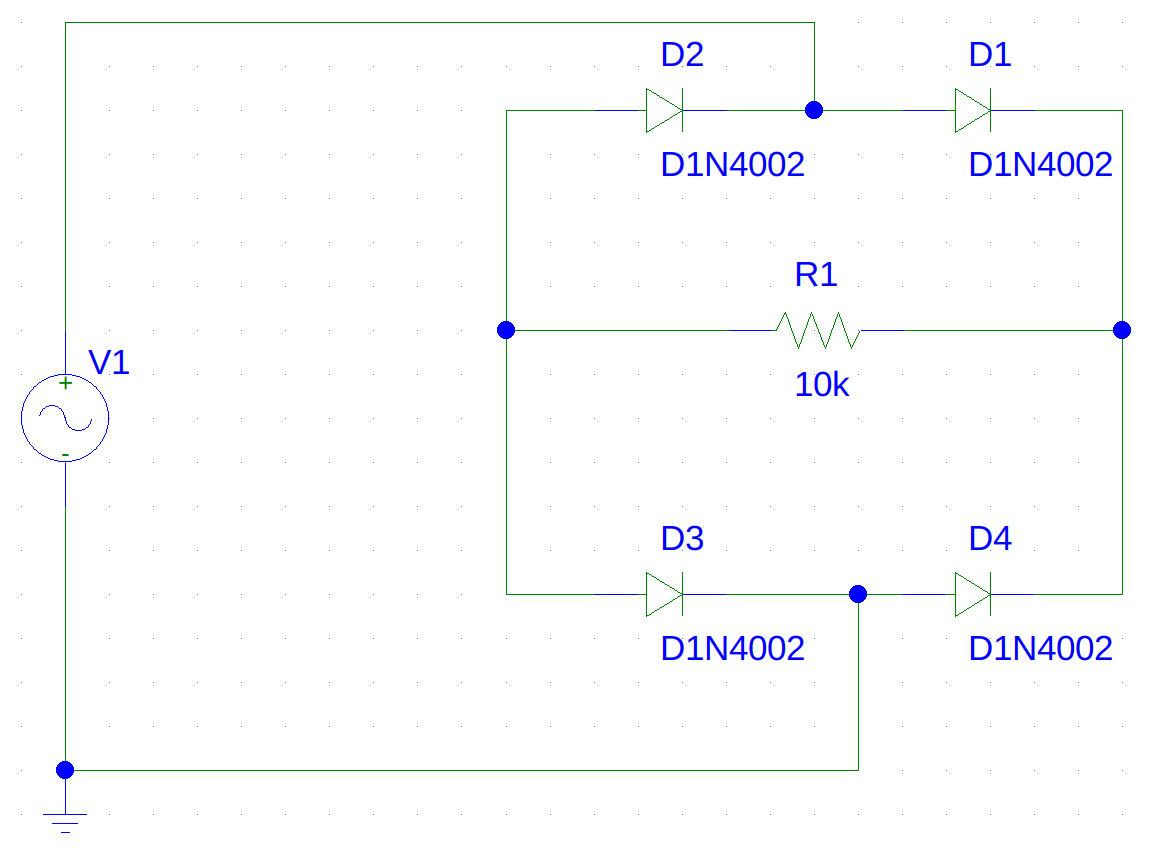
\includegraphics[width=0.8\textwidth]{schematic_no_filter.png}
		\caption{PSpice schematic of the full-wave bridge rectifier without
			filter capacitor ($R_1 = \SI{100}{\kilo\ohm}$,
			$V_{\mathrm{in}} = \SI{100}{\volt}$ amplitude at \SI{50}{\hertz})}
		\label{fig:sch1}
	\end{figure}
	
	\begin{figure}[H]
		\centering
		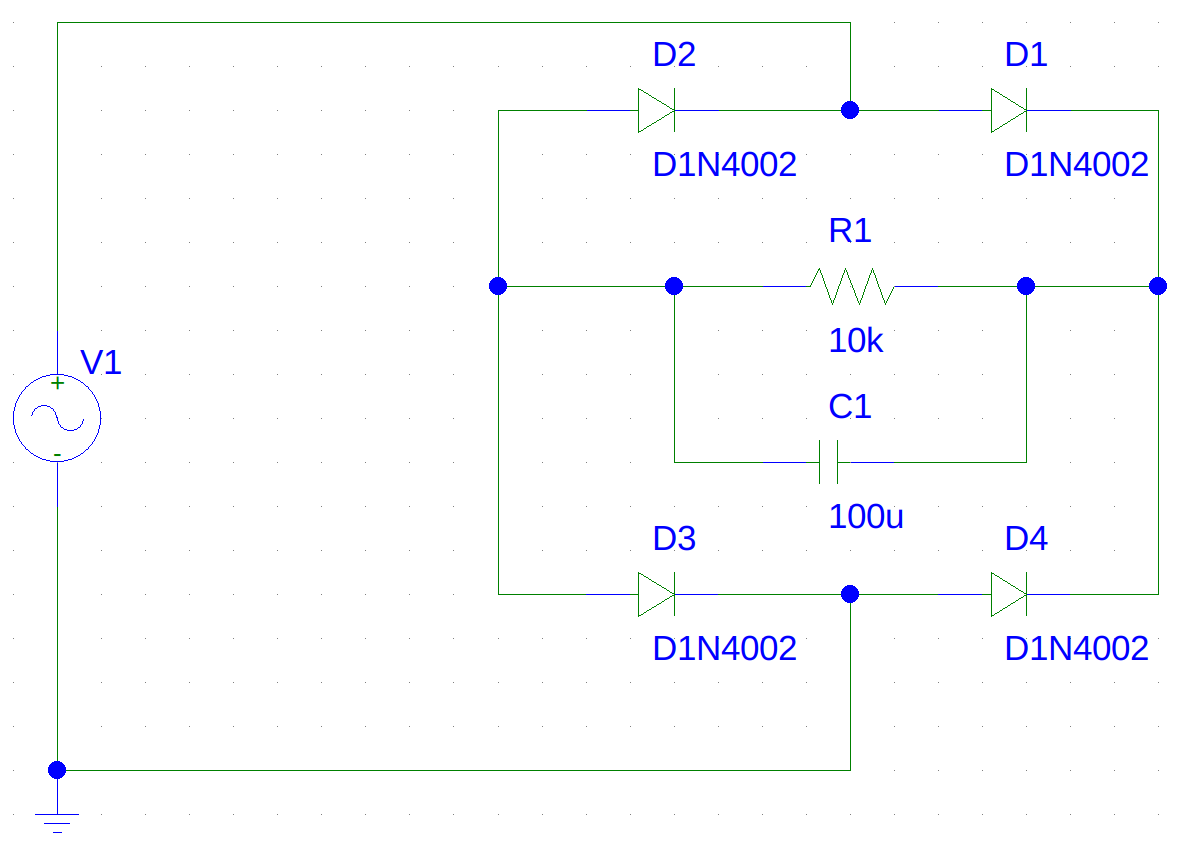
\includegraphics[width=0.8\textwidth]{schematic_with_capacitor.png}
		\caption{PSpice schematic of the full-wave bridge rectifier with
			filter capacitor ($C_1 = \SI{100}{\micro\farad}$ in parallel with
			$R_1 = \SI{100}{\kilo\ohm}$)}
		\label{fig:sch2}
	\end{figure}
	
	\begin{figure}[H]
		\centering
		\includegraphics[width=0.8\textwidth]{schematic_with_capacitor_modified.png}
		\caption{PSpice schematic of the modified bridge rectifier (task 4,
			filter capacitor changed to $C_1 = \SI{10}{\micro\farad}$)}
		\label{fig:sch3}
	\end{figure}
	
	\subsection{PSpice netlist code}
	The same circuits were described in PSpice netlist form; each netlist was stored as a \texttt{.cir} file and simulated with a transient analysis of \SI{100}{\milli\second} for the unfiltered circuit and \SI{300}{\milli\second} for the filtered ones, using a \SI{10}{\micro\second} print step. The netlists of the unfiltered circuit and of the \SI{100}{\micro\farad} filtered circuit are listed below; the modified circuit of task 4 differs from the latter only in the capacitor statement.
	
	\textbf{Circuit 1 (without filter capacitor):}
	{\small
		\begin{verbatim}
* Full-Wave Bridge Rectifier without Filter Capacitor
V1 1 0 SIN(0 100 50)
D1 1 2 D1N914
D2 0 2 D1N914
D3 3 1 D1N914
D4 3 0 D1N914
R1 2 3 100K
.MODEL D1N914 D
.TRAN 10US 100MS
.PROBE
.END
	\end{verbatim}}
	
	\textbf{Circuit 2 (with filter capacitor):}
	{\small
		\begin{verbatim}
* Full-Wave Bridge Rectifier with Filter Capacitor
VS 1 0 SIN(0 100 50)
D1 1 2 D1N914
D2 0 2 D1N914
D3 3 1 D1N914
D4 3 0 D1N914
C1 2 3 100U
R1 2 3 100K
.MODEL D1N914 D
.TRAN 10US 300MS
.PROBE
.END
	\end{verbatim}}
	
	
	% =====================================================================
	\section{Simulation/Working Procedure}
	
	PSpice was used to construct the circuits, run the transient simulations, and display the waveforms in the Probe waveform viewer. The work was divided into the following three parts.
	
	\subsection*{Part 1: Entering the circuit through the schematic editor}
	
	\begin{enumerate}[leftmargin=0.8cm,label=\textbf{Step \arabic*:},itemsep=0.55em]
		\item \textbf{Draw the schematic.}
		Open PSpice Schematics and select \texttt{Draw $\rightarrow$ Get New Part} (or press \texttt{Ctrl+G}). Place the four diodes (D1N914), the load resistor $R_1$, the filter capacitor $C_1$, the sinusoidal voltage source VSIN, and the ground symbol on the workspace. Connect them with \texttt{Draw $\rightarrow$ Wire} (\texttt{Ctrl+W}) so that the bridge, the load, and the source match the theory diagrams of Figs.~\ref{fig:bridge-theory} and \ref{fig:bridge-filter} and the schematics of Figs.~\ref{fig:sch1}--\ref{fig:sch3}.
		
		\item \textbf{Assign the component values.}
		Double-click each component and enter its attributes: $R_1 = \SI{100}{\kilo\ohm}$ for all three circuits; $C_1 = \SI{100}{\micro\farad}$ (later changed to \SI{10}{\micro\farad} for task 4); and for the VSIN source set the DC offset $V_{\mathrm{OFF}} = \SI{0}{\volt}$, the amplitude $V_{\mathrm{AMPL}} = \SI{100}{\volt}$, and the frequency $\mathrm{FREQ} = \SI{50}{\hertz}$. Save the schematic under an identifiable name.
		
		\item \textbf{Set up the transient analysis.}
		Select \texttt{Analysis $\rightarrow$ Setup}, enable \texttt{Transient}, and enter a print step of \SI{10}{\micro\second} and a final time of \SI{100}{\milli\second} for the unfiltered circuit and \SI{300}{\milli\second} for the two filtered circuits, i.e.\ five and fifteen input periods, long enough for the slow filter charge-up to settle before the readings are taken.
	\end{enumerate}
	
	\subsection*{Part 2: Entering the circuit through the netlist}
	
	\begin{enumerate}[leftmargin=0.8cm,label=\textbf{Step \arabic*:},itemsep=0.55em]
		\setcounter{enumi}{3}
		\item \textbf{Type the netlist.}
		As an equivalent alternative to the schematic entry, create a text file with a \texttt{.cir} extension and type the netlist exactly as listed in Section 4.4: a title line, the source statement \texttt{VS 1 0 SIN(0 100 50)}, the four diode statements with the D1N914 model, the load branch (\texttt{R1} and, for the filtered circuits, \texttt{C1}), the \texttt{.MODEL} line, the \texttt{.TRAN} command, and \texttt{.PROBE}/\texttt{.END}. Run the netlist through the PSpice A/D simulator.
	\end{enumerate}
	
	\subsection*{Part 3: Running the simulation and reading the waveforms}
	
	\begin{enumerate}[leftmargin=0.8cm,label=\textbf{Step \arabic*:},itemsep=0.55em]
		\setcounter{enumi}{4}
		\item \textbf{Run the simulation and display the traces.}
		Start the simulation (\texttt{Analysis} $\rightarrow$ \texttt{Simulate}, or \texttt{F11}). When the Probe window opens, add the input-voltage trace \texttt{V(1)}, the load-voltage trace \texttt{V(R1:1,R1:2)}, and, for the unfiltered circuit, the diode-voltage trace \texttt{V(D2:1,D2:2)} through \texttt{Trace $\rightarrow$ Add Trace}. Repeat for all three circuits.
		
		\item \textbf{Read the waveform values with the cursor.}
		Enable the cursor (\texttt{Trace $\rightarrow$ Cursor $\rightarrow$ Display}). Read the input peak, the output peak, and the output valley on the last steady-state output period, and determine the peak-to-peak ripple from the difference between the output maximum and minimum. Measure the DC (average) value and the RMS value over one full output period, i.e.\ the interval between two successive output minima, using the waveform viewer's average and RMS measurement functions. Read the output frequency from the time between two successive output maxima.
		
		\item \textbf{Tabulate and compare.}
		Record the values read from the waveform viewer for the three circuits, calculate the corresponding theoretical values from Section 4.6, and evaluate the percentage error using Eq.~\eqref{eq:percentage-error}.
	\end{enumerate}
	
	% =====================================================================
	\section{Calculation}
	% =====================================================================
	The given values are: $V_m = \SI{100}{\volt}$, $f = \SI{50}{\hertz}$ ($T = \SI{20}{\milli\second}$), $R_1 = \SI{100}{\kilo\ohm}$ for all three circuits, $V_D = \SI{0.7}{\volt}$ per silicon diode (so $2V_D = \SI{1.4}{\volt}$), $C_1 = \SI{100}{\micro\farad}$ for the filtered circuit and $C_1 = \SI{10}{\micro\farad}$ for the modified circuit of task 4.

	\textbf{Without filter capacitor.} From \eqref{eq:vp-out},
	\begin{equation}
		V_{p(\mathrm{out})} = V_m - 2V_D = 100 - 1.4 = \SI{98.6}{\volt},
		\label{eq:calc-vp}
	\end{equation}
	and the peak output current is
	\begin{equation}
		I_{p(\mathrm{out})} = \frac{V_{p(\mathrm{out})}}{R_1}
		= \frac{98.6}{10^{5}} = \SI{0.986}{\milli\ampere}.
		\label{eq:calc-ipk}
	\end{equation}
	From \eqref{eq:vdc} and \eqref{eq:vrms},
	\begin{equation}
		V_{\mathrm{dc}} = \frac{2 \times 98.6}{\pi} = \SI{62.77}{\volt},
		\qquad
		I_{\mathrm{dc}} = \frac{62.77}{10^{5}} = \SI{0.628}{\milli\ampere},
		\label{eq:calc-vdc}
	\end{equation}
	\begin{equation}
		V_{\mathrm{rms}} = \frac{98.6}{\sqrt{2}} = \SI{69.73}{\volt},
		\qquad
		I_{\mathrm{rms}} = \frac{69.73}{10^{5}} = \SI{0.697}{\milli\ampere}.
		\label{eq:calc-vrms}
	\end{equation}
	The output powers follow from \eqref{eq:powers}:
	\begin{equation}
		P_{\mathrm{dc}} = (0.6277\times 10^{-3})^{2}\times 10^{5} = \SI{39.40}{\milli\watt},
		\qquad
		P_{\mathrm{ac}} = (0.6973\times 10^{-3})^{2}\times 10^{5} = \SI{48.61}{\milli\watt}.
		\label{eq:calc-powers}
	\end{equation}
	Hence, from \eqref{eq:eta-ff-r},
	\begin{equation}
		\eta = \frac{39.40}{48.61}\times 100\% = 81.06\%,
		\qquad
		FF = \frac{69.73}{62.77} = 1.111,
		\qquad
		r = \sqrt{1.111^{2}-1} = 0.483 .
		\label{eq:calc-eta}
	\end{equation}
	The peak inverse voltage per diode is $PIV \approx V_m = \SI{100}{\volt}$, and the output frequency is $f_{\mathrm{out}} = 2f = \SI{100}{\hertz}$.
	
	\textbf{With filter capacitor ($C_1 = \SI{100}{\micro\farad}$).} The capacitor charges approximately to the peak output voltage, $V_{p(\mathrm{cap})} = V_m - 2V_D = \SI{98.6}{\volt}$. Since $I_L \approx V_{\mathrm{dc}}/R_1$, Eq.~\eqref{eq:ripple-estimates} gives $V_{r(pp)} \approx V_{\mathrm{dc}}/(2fC_1R_1)$. Substituting into $V_{\mathrm{dc}} \approx V_{p(\mathrm{out})} - V_{r(pp)}/2$ yields the self-consistent solution
	\begin{equation}
		V_{\mathrm{dc}}\left(1 + \frac{1}{4fC_1R_1}\right) = V_{p(\mathrm{out})}.
		\label{eq:self-consistent}
	\end{equation}
	With $4fC_1R_1 = 4\times 50\times 100\times 10^{-6}\times 100\times 10^{3} = 2000$:
	\begin{equation}
		V_{\mathrm{dc}} = \frac{98.6}{1 + 1/2000} = \SI{98.55}{\volt},
		\qquad
		V_{r(pp)} = \frac{98.55}{1000} = \SI{0.0986}{\volt}.
		\label{eq:calc-vdc-100u}
	\end{equation}
	The load current is $I_L = V_{\mathrm{dc}}/R_1 = \SI{0.9855}{\milli\ampere}$, the RMS ripple is
	\begin{equation}
		V_{r(\mathrm{rms})} = \frac{0.0986}{2\sqrt{3}} = \SI{0.0285}{\volt},
		\qquad
		r = \frac{0.0285}{98.55} = 0.000289,
		\label{eq:calc-r-100u}
	\end{equation}
	so the percentage ripple is $\%r = 0.0289\%$, and the ripple frequency is $f_r = 2f = \SI{100}{\hertz}$.
	
	\textbf{With modified filter capacitor ($C_1 = \SI{10}{\micro\farad}$, task 4).} Now $4fC_1R_1 = 4\times 50\times 10\times 10^{-6}\times 100\times 10^{3} = 200$, so
	\begin{equation}
		V_{\mathrm{dc}} = \frac{98.6}{1 + 1/200} = \SI{98.11}{\volt},
		\qquad
		V_{r(pp)} = \frac{98.11}{100} = \SI{0.981}{\volt},
		\label{eq:calc-vdc-10u}
	\end{equation}
	\begin{equation}
		V_{r(\mathrm{rms})} = \frac{0.981}{2\sqrt{3}} = \SI{0.283}{\volt},
		\qquad
		r = \frac{0.283}{98.11} = 0.00289 ,
		\label{eq:calc-r-10u}
	\end{equation}
	so the percentage ripple is $\%r = 0.289\%$. Here the discharge time constant $R_1C_1 = \SI{1}{\second}$ is one hundred times the half-period $T/2$ (and \SI{10}{\second}, one thousand times, for $C_1 = \SI{100}{\micro\farad}$), so the small-ripple assumption $R_1C_1 \gg T/2$ behind Eqs.~\eqref{eq:ripple-estimates} and \eqref{eq:r-filtered} is comfortably satisfied for both filtered circuits.
	
	% =====================================================================
	\section{Result Analysis}
	% =====================================================================
	\subsection{Simulated waveforms}
	Figures~\ref{fig:wave1}--\ref{fig:wave3} show the input and output voltage waveforms obtained from the PSpice simulations. In all three circuits the input (violet trace, \texttt{V(1)}) is the \SI{100}{\volt}, \SI{50}{\hertz} sinusoid, and the green trace is the load voltage \texttt{V(R1:1,R1:2)}.
	
	\begin{figure}[H]
		\centering
		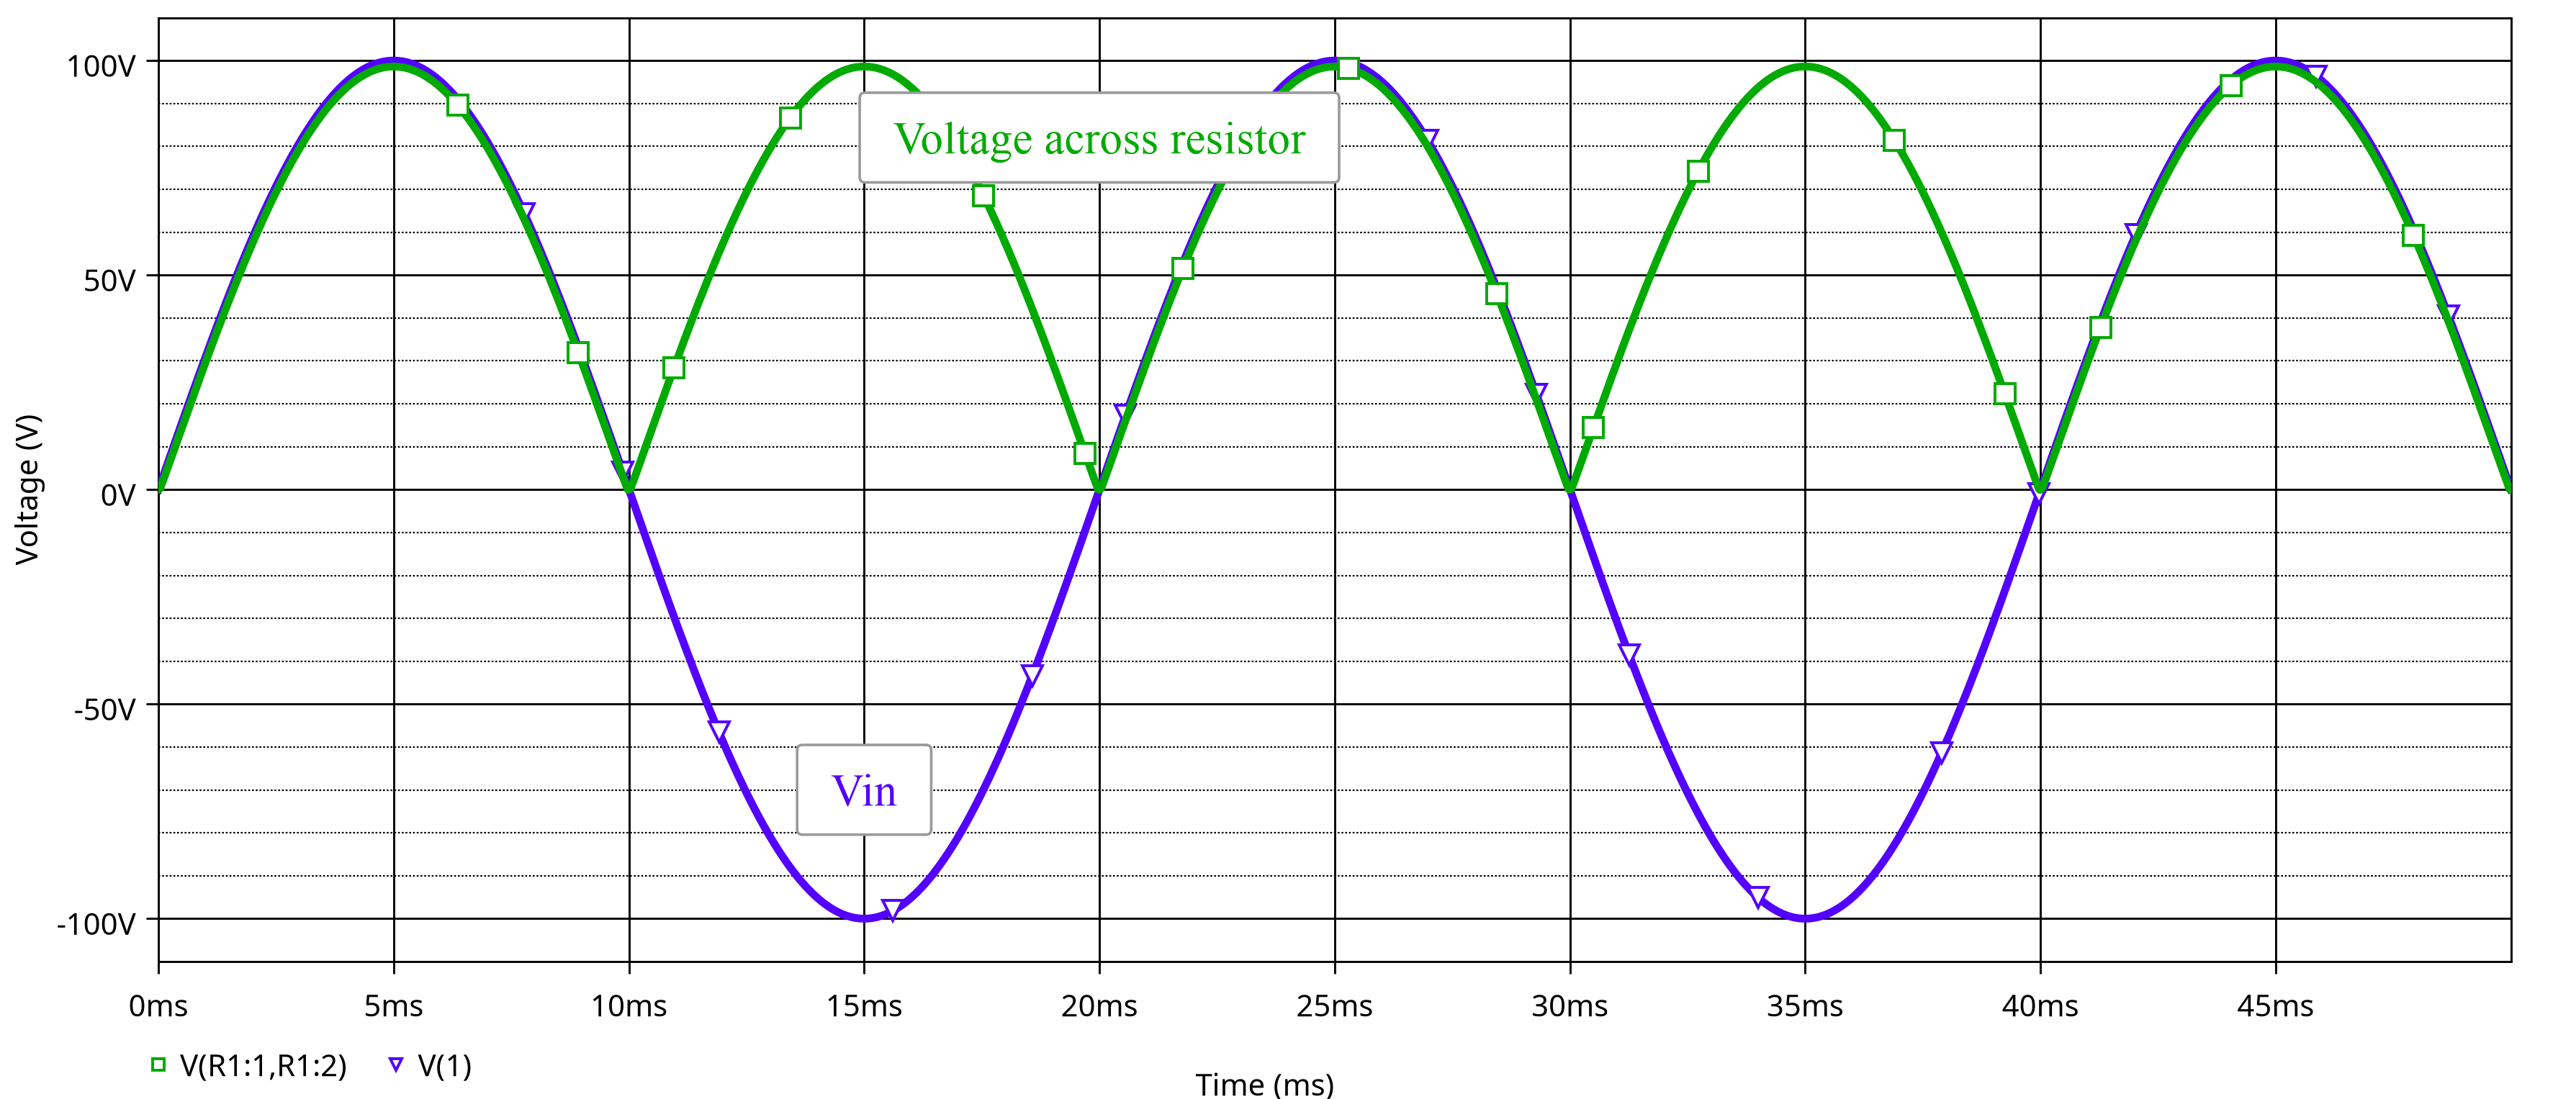
\includegraphics[width=0.95\textwidth]{full_bridge.png}
		\caption{PSpice output: input and load-voltage waveforms of the
			bridge rectifier without filter capacitor}
		\label{fig:wave1}
	\end{figure}
	
	\begin{figure}[H]
		\centering
		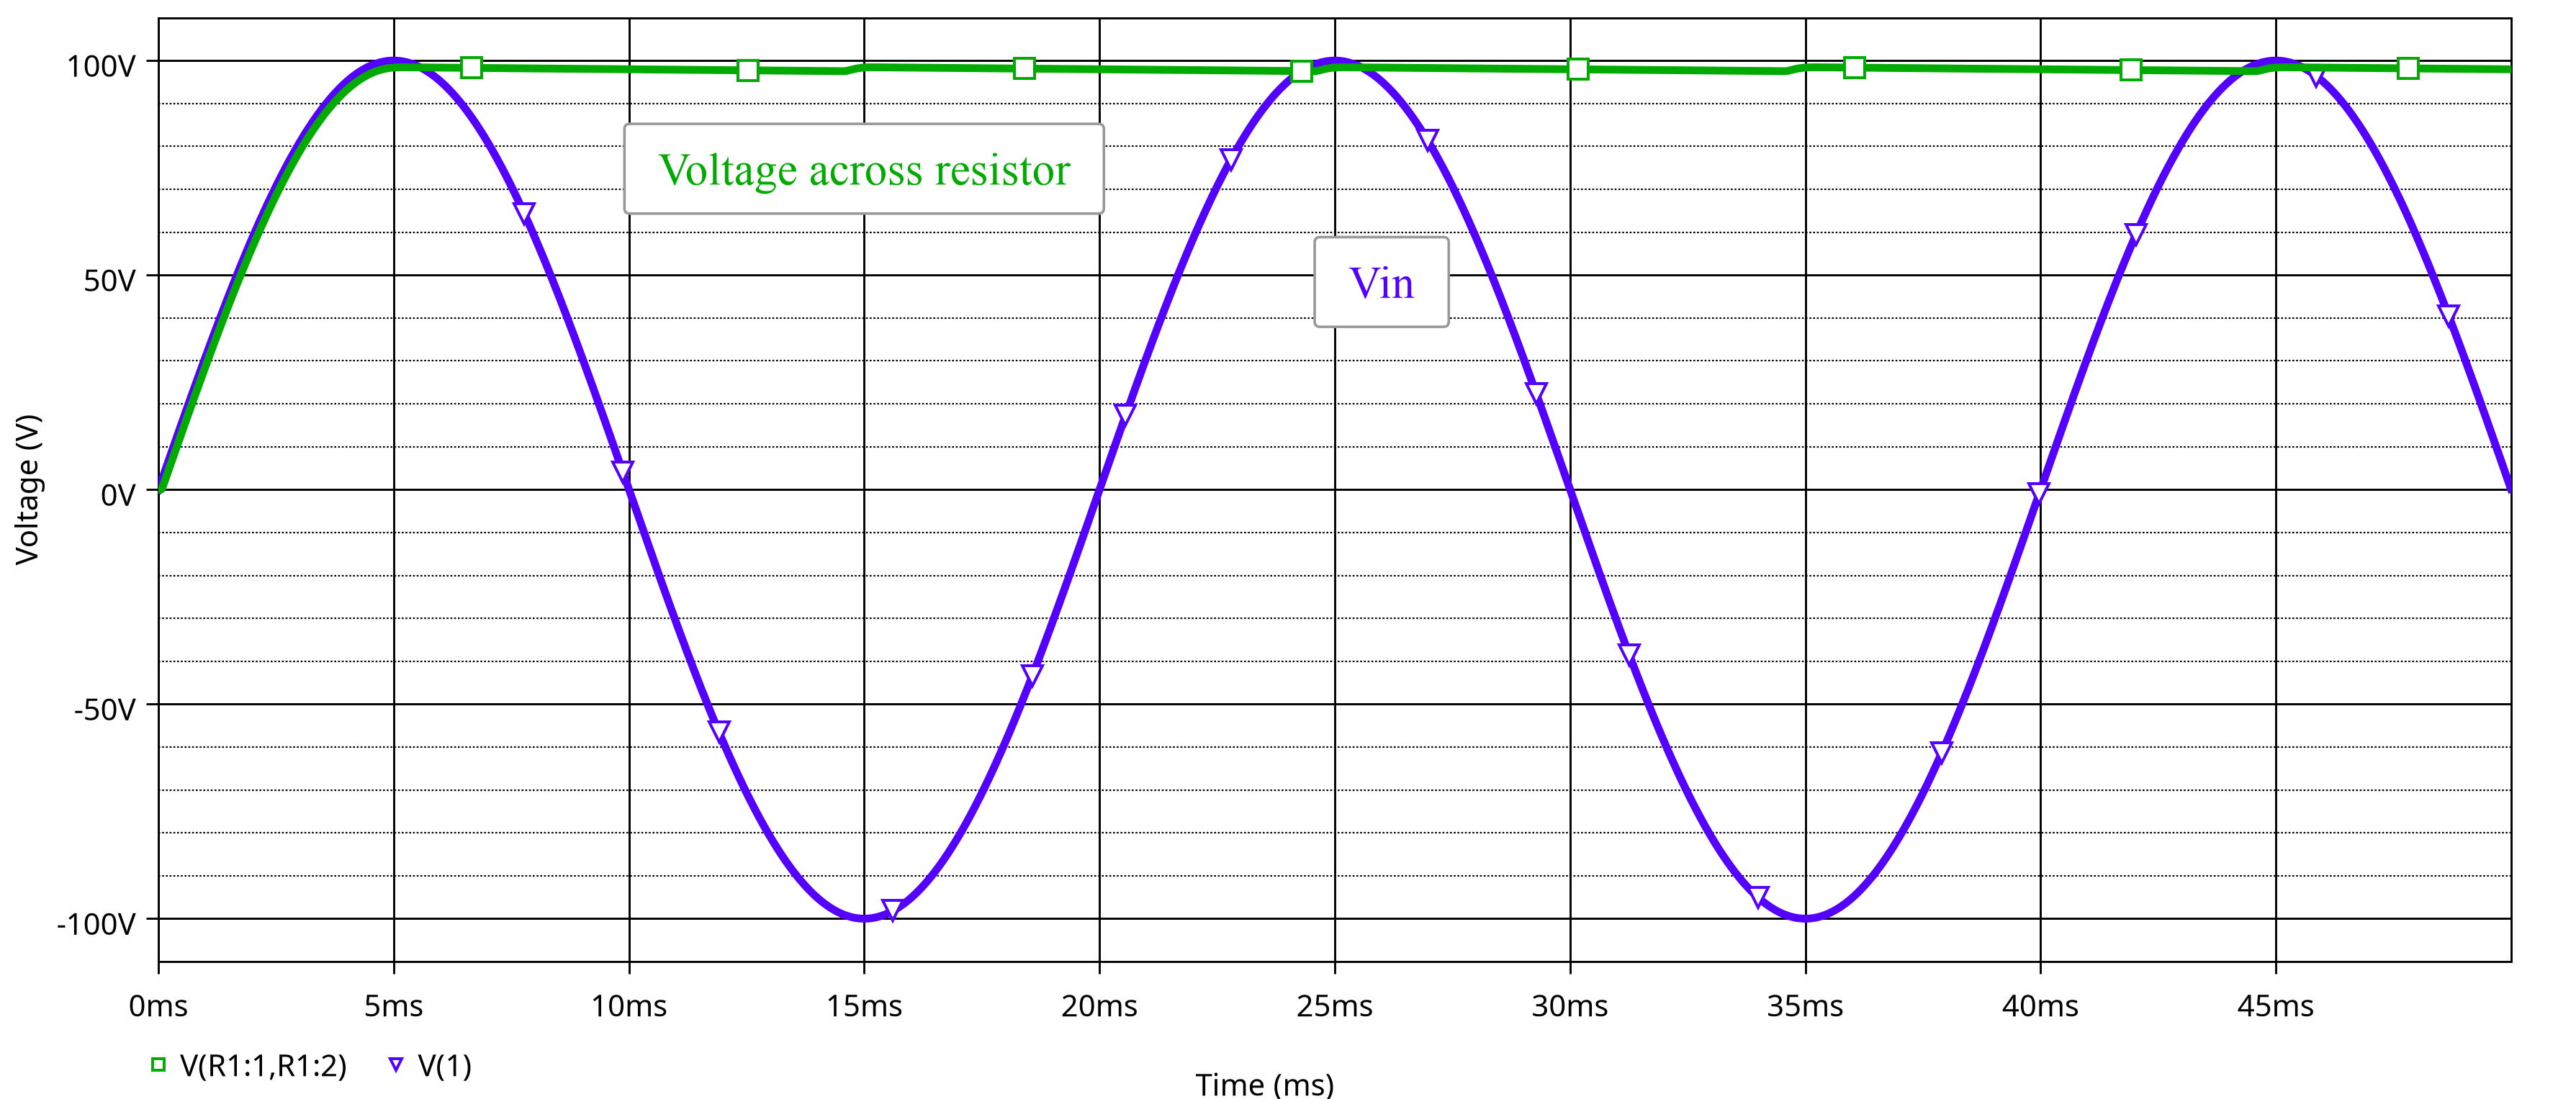
\includegraphics[width=0.95\textwidth]{full_bridge_with_capacitor.png}
		\caption{PSpice output: input and load-voltage waveforms of the
			bridge rectifier with $C_1 = \SI{100}{\micro\farad}$}
		\label{fig:wave2}
	\end{figure}
	
	\begin{figure}[H]
		\centering
		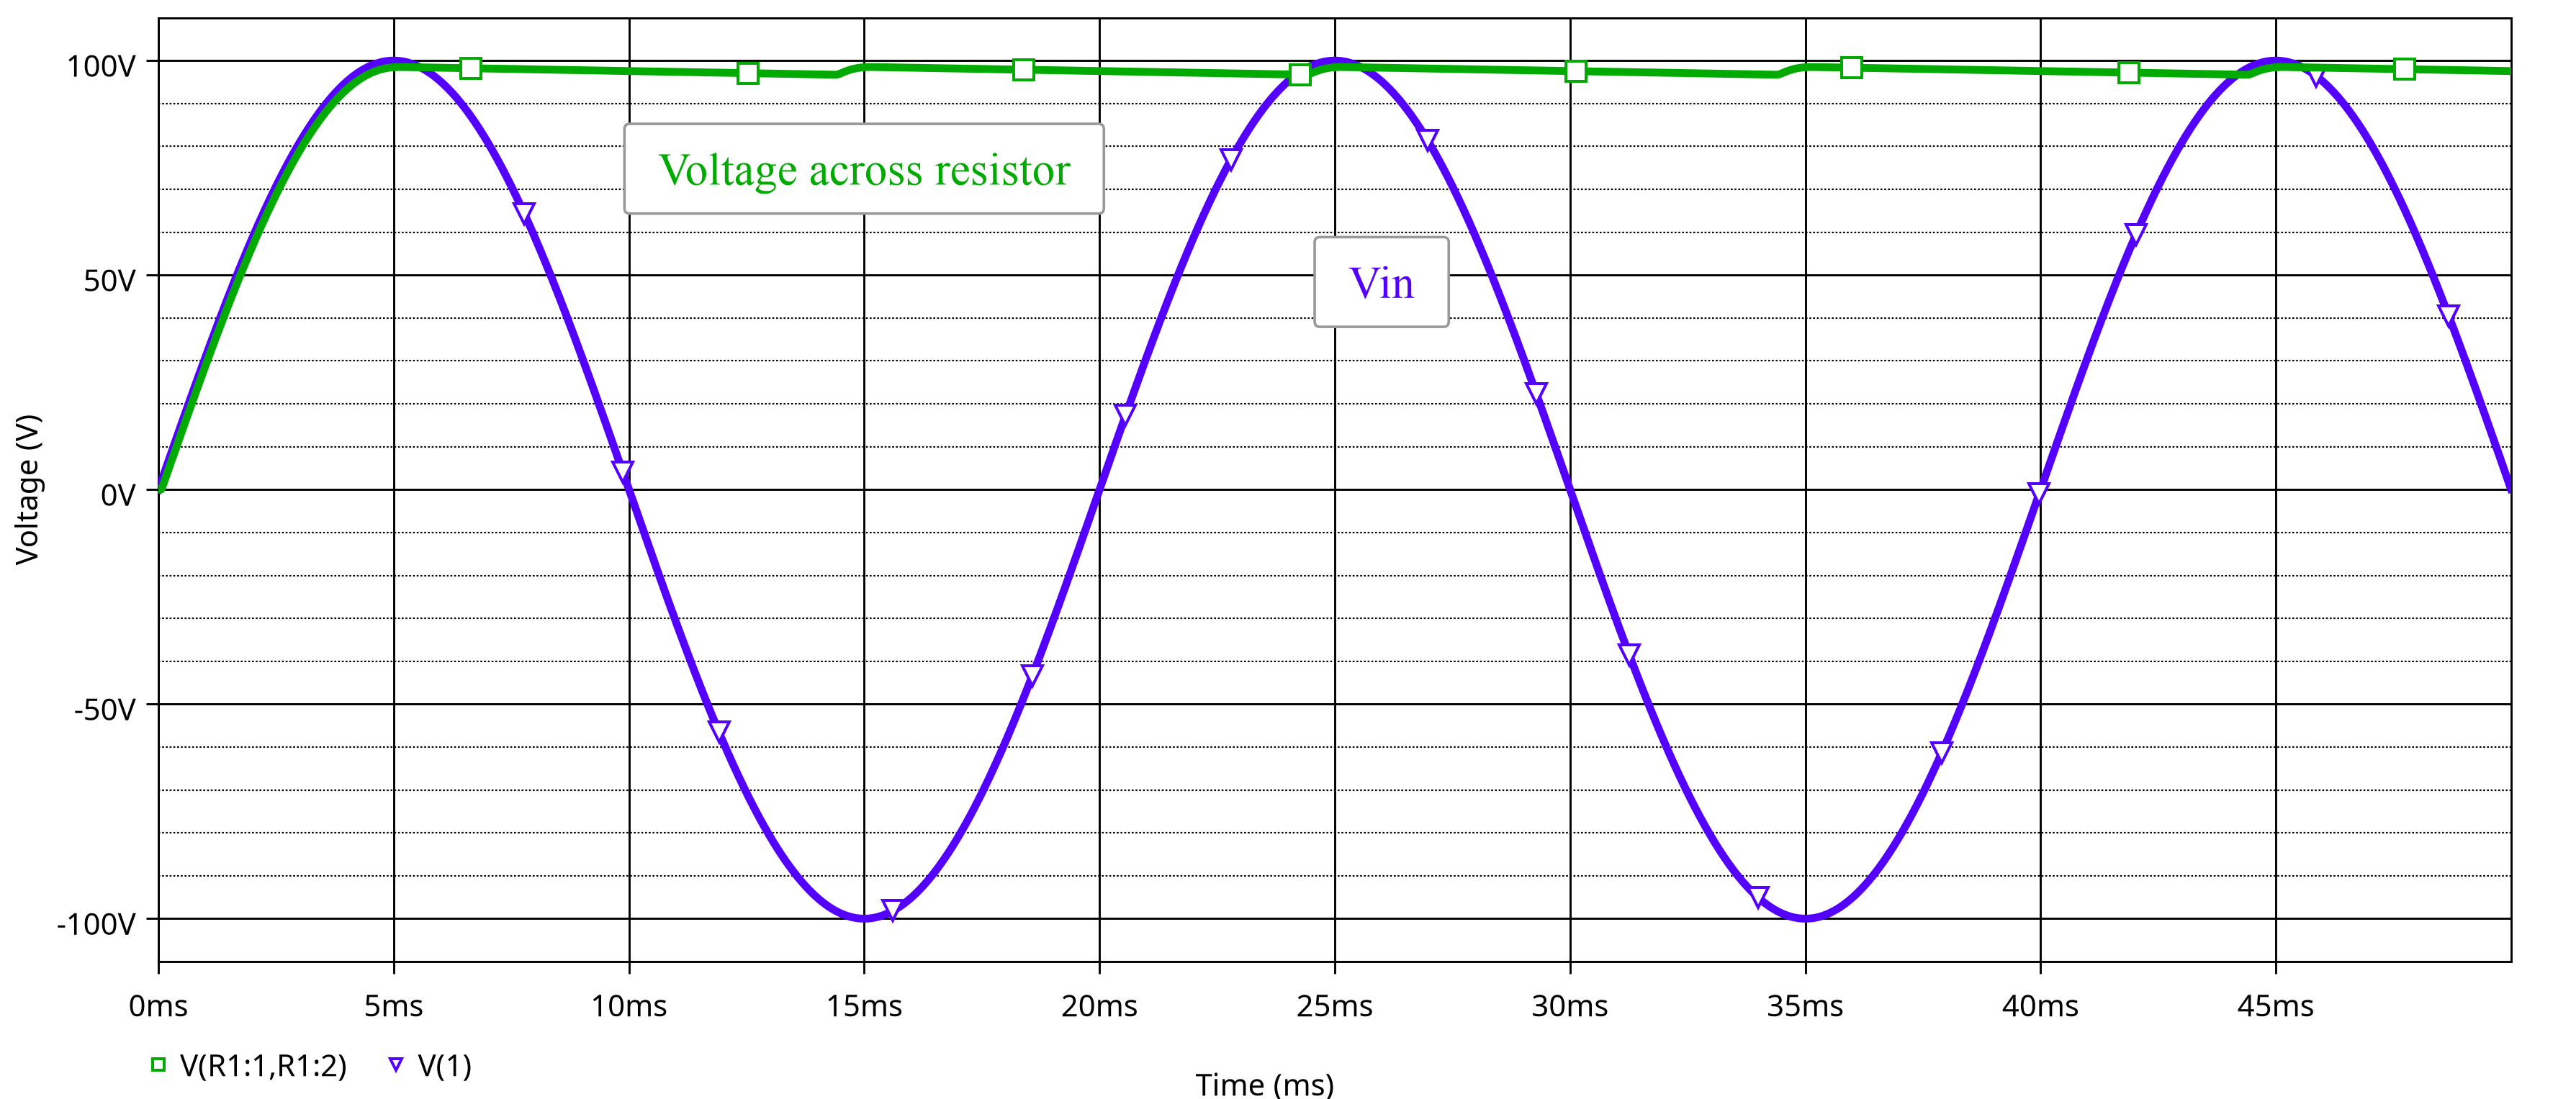
\includegraphics[width=0.95\textwidth]{full_bridge_with_capacitor_changed.png}
		\caption{PSpice output: input and load-voltage waveforms of the
			bridge rectifier with the modified $C_1 = \SI{10}{\micro\farad}$
			(task 4)}
		\label{fig:wave3}
	\end{figure}
	
	Without the capacitor (Figure~\ref{fig:wave1}) the output is a full-wave rectified waveform: the negative input half-cycles are flipped positive, the output period is \SI{10}{\milli\second} (i.e.\ $f_{\mathrm{out}} = \SI{100}{\hertz}$), and the output returns to approximately \SI{0}{\volt} between humps, where for a brief interval no diode pair conducts; the humps peak at \SI{98.28}{\volt} against the \SI{100}{\volt} input crests, the difference being the total drop of the two conducting diodes. With $R_1 = \SI{100}{\kilo\ohm}$ the filtered circuits draw only about \SI{1}{\milli\ampere}, so the capacitor discharges very little between recharges; both outputs (Figs.~\ref{fig:wave2} and \ref{fig:wave3}) also show the capacitor's initial charge-up over the first few input cycles, after which they sit almost flat just below the \SI{100}{\volt} crests, with steady-state ripples of only \SI{0.092}{\volt} ($C_1 = \SI{100}{\micro\farad}$) and \SI{0.87}{\volt} ($C_1 = \SI{10}{\micro\farad}$, task 4).
	
	\subsection{Simulated parameters read from the waveforms}
	The quantities read from the Probe traces with the cursor are compared below with the theoretical values calculated in Section 4.6. Table~\ref{tab:compare-1} refers to the circuit without filter capacitor. The total diode drop read at the output peak is the difference between the input and output peaks, $2V_D = V_m - V_{p(\mathrm{out})}$; the peak inverse voltage is the largest voltage appearing across a diode and is read from the diode-voltage trace \texttt{V(D2:1,D2:2)} over the half-cycle in which the opposite pair conducts.
	
	\begin{table}[H]
		\centering
		\caption{Theoretical versus simulated parameters of the bridge
			rectifier without filter capacitor}
		\label{tab:compare-1}
		\footnotesize
		\renewcommand{\arraystretch}{1.2}
		\setlength{\tabcolsep}{3pt}
		\begin{tabular}{|l|l|l|c|c|c|}
			\hline
			\rowcolor{black!12}\textbf{Quantity} & \textbf{Formula} & \textbf{Calculation} & \textbf{Theoretical} & \textbf{Simulated} & \textbf{\% Error} \\
			\hline
			Peak input voltage & $V_m$ & given & \SI{100}{\volt} & \SI{100.0}{\volt} & $0.00$ \\
			\hline
			Total diode drop & $2V_D$ & $2\times 0.7$ & \SI{1.4}{\volt} & \SI{1.72}{\volt} & $23.01$ \\
			\hline
			Peak output voltage & $V_m - 2V_D$ & $100 - 1.4$ & \SI{98.6}{\volt} & \SI{98.28}{\volt} & $0.33$ \\
			\hline
			Peak output current & $(V_m - 2V_D)/R_1$ & $98.6/10^{5}$ & \SI{0.986}{\milli\ampere} & \SI{0.983}{\milli\ampere} & $0.33$ \\
			\hline
			DC output voltage & $2(V_m - 2V_D)/\pi$ & $2\times 98.6/\pi$ & \SI{62.77}{\volt} & \SI{62.12}{\volt} & $1.04$ \\
			\hline
			DC load current & $V_{\mathrm{dc}}/R_1$ & $62.77/10^{5}$ & \SI{0.628}{\milli\ampere} & \SI{0.621}{\milli\ampere} & $1.04$ \\
			\hline
			RMS output voltage & $(V_m - 2V_D)/\sqrt{2}$ & $98.6/\sqrt{2}$ & \SI{69.73}{\volt} & \SI{69.25}{\volt} & $0.67$ \\
			\hline
			RMS load current & $V_{\mathrm{rms}}/R_1$ & $69.73/10^{5}$ & \SI{0.697}{\milli\ampere} & \SI{0.693}{\milli\ampere} & $0.67$ \\
			\hline
			DC output power & $I_{\mathrm{dc}}^{2}R_1$ & $0.6277^{2}\times 100$ & \SI{39.40}{\milli\watt} & \SI{38.59}{\milli\watt} & $2.06$ \\
			\hline
			AC load power & $I_{\mathrm{rms}}^{2}R_1$ & $0.6973^{2}\times 100$ & \SI{48.61}{\milli\watt} & \SI{47.96}{\milli\watt} & $1.35$ \\
			\hline
			Efficiency & $(P_{\mathrm{dc}}/P_{\mathrm{ac}})\times 100\%$ & $(39.40/48.61)\times 100\%$ & $81.06\%$ & $80.47\%$ & $0.73$ \\
			\hline
			Form factor & $V_{\mathrm{rms}}/V_{\mathrm{dc}}$ & $69.73/62.77$ & $1.111$ & $1.115$ & $0.37$ \\
			\hline
			Ripple factor & $\sqrt{(V_{\mathrm{rms}}/V_{\mathrm{dc}})^{2}-1}$ & $\sqrt{1.111^{2}-1}$ & $0.483$ & $0.493$ & $1.92$ \\
			\hline
			Peak inverse voltage & $\approx V_m$ & given & \SI{100}{\volt} & \SI{99.14}{\volt} & $0.86$ \\
			\hline
			Output frequency & $2f$ & $2\times 50$ & \SI{100}{\hertz} & \SI{99.92}{\hertz} & $0.08$ \\
			\hline
		\end{tabular}
	\end{table}
	
	Tables~\ref{tab:compare-2} and \ref{tab:compare-3} refer to the filtered circuits. The peak capacitor voltage equals the output maximum, the output valley is the minimum to which the capacitor discharges between recharges, and the ripple quantities are read from the last steady-state output period.
	
	\begin{table}[H]
		\centering
		\caption{Theoretical versus simulated parameters of the bridge
			rectifier with $C_1 = \SI{100}{\micro\farad}$}
		\label{tab:compare-2}
		\footnotesize
		\renewcommand{\arraystretch}{1.2}
		\setlength{\tabcolsep}{3pt}
		\begin{tabular}{|l|l|l|c|c|c|}
			\hline
			\rowcolor{black!12}\textbf{Quantity} & \textbf{Formula} & \textbf{Calculation} & \textbf{Theoretical} & \textbf{Simulated} & \textbf{\% Error} \\
			\hline
			Peak capacitor voltage & $\approx V_m - 2V_D$ & $100 - 1.4$ & \SI{98.6}{\volt} & \SI{98.00}{\volt} & $0.61$ \\
			\hline
			Ripple frequency & $= 2f$ & $2\times 50$ & \SI{100}{\hertz} & \SI{100.06}{\hertz} & $0.06$ \\
			\hline
			Peak-to-peak ripple voltage & $\approx I_L/(2fC_1)$ & $98.55/1000$ & \SI{0.0986}{\volt} & \SI{0.0920}{\volt} & $6.62$ \\
			\hline
			RMS ripple voltage & $= V_{r(pp)}/(2\sqrt{3})$ & $0.0986/(2\sqrt{3})$ & \SI{0.0285}{\volt} & \SI{0.0276}{\volt} & $2.84$ \\
			\hline
			Average/DC output voltage & $\approx V_{p(\mathrm{cap})} - V_{r(pp)}/2$ & $98.6/(1+1/2000)$ & \SI{98.55}{\volt} & \SI{97.96}{\volt} & $0.60$ \\
			\hline
			Load current & $\approx V_{\mathrm{dc}}/R_1$ & $98.55/10^{5}$ & \SI{0.9855}{\milli\ampere} & \SI{0.980}{\milli\ampere} & $0.60$ \\
			\hline
			Ripple factor & $= V_{r(\mathrm{rms})}/V_{\mathrm{dc}}$ & $0.0285/98.55$ & $0.000289$ & $0.000282$ & $2.25$ \\
			\hline
			Percentage ripple & $= r\times 100\%$ & $0.000289\times 100$ & $0.0289\%$ & $0.0282\%$ & $2.25$ \\
			\hline
		\end{tabular}
	\end{table}
	
	\begin{table}[H]
		\centering
		\caption{Theoretical versus simulated parameters of the bridge
			rectifier with the modified $C_1 = \SI{10}{\micro\farad}$ (task 4)}
		\label{tab:compare-3}
		\footnotesize
		\renewcommand{\arraystretch}{1.2}
		\setlength{\tabcolsep}{3pt}
		\begin{tabular}{|l|l|l|c|c|c|}
			\hline
			\rowcolor{black!12}\textbf{Quantity} & \textbf{Formula} & \textbf{Calculation} & \textbf{Theoretical} & \textbf{Simulated} & \textbf{\% Error} \\
			\hline
			Peak capacitor voltage & $\approx V_m - 2V_D$ & $100 - 1.4$ & \SI{98.6}{\volt} & \SI{98.15}{\volt} & $0.46$ \\
			\hline
			Ripple frequency & $= 2f$ & $2\times 50$ & \SI{100}{\hertz} & \SI{100.04}{\hertz} & $0.04$ \\
			\hline
			Peak-to-peak ripple voltage & $\approx I_L/(2fC_1)$ & $98.11/100$ & \SI{0.9811}{\volt} & \SI{0.8669}{\volt} & $11.64$ \\
			\hline
			RMS ripple voltage & $= V_{r(pp)}/(2\sqrt{3})$ & $0.9811/(2\sqrt{3})$ & \SI{0.2832}{\volt} & \SI{0.2605}{\volt} & $8.03$ \\
			\hline
			Average/DC output voltage & $\approx V_{p(\mathrm{cap})} - V_{r(pp)}/2$ & $98.6/(1+1/200)$ & \SI{98.11}{\volt} & \SI{97.72}{\volt} & $0.40$ \\
			\hline
			Load current & $\approx V_{\mathrm{dc}}/R_1$ & $98.11/10^{5}$ & \SI{0.9811}{\milli\ampere} & \SI{0.977}{\milli\ampere} & $0.40$ \\
			\hline
			Ripple factor & $= V_{r(\mathrm{rms})}/V_{\mathrm{dc}}$ & $0.2832/98.11$ & $0.00289$ & $0.00267$ & $7.66$ \\
			\hline
			Percentage ripple & $= r\times 100\%$ & $0.00289\times 100$ & $0.289\%$ & $0.267\%$ & $7.66$ \\
			\hline
		\end{tabular}
	\end{table}
	
	\subsection{Effect of changing the filter capacitance (task 4)}
	Table~\ref{tab:task4} summarizes the simulated effect of reducing the filter capacitor from \SI{100}{\micro\farad} to \SI{10}{\micro\farad} while everything else is unchanged.
	
	\begin{table}[H]
		\centering
		\caption{Simulated output of the filtered rectifier before and after
			changing the filter capacitance}
		\label{tab:task4}
		\renewcommand{\arraystretch}{1.25}
		\begin{tabular}{|l|c|c|}
			\hline
			\rowcolor{black!12}\textbf{Quantity} & \textbf{$C_1 = \SI{100}{\micro\farad}$} & \textbf{$C_1 = \SI{10}{\micro\farad}$} \\
			\hline
			Discharge time constant $R_1C_1$ & \SI{10}{\second} ($1000\times T/2$) & \SI{1}{\second} ($100\times T/2$) \\
			\hline
			Simulated output peak & \SI{98.00}{\volt} & \SI{98.15}{\volt} \\
			\hline
			Simulated output valley & \SI{97.91}{\volt} & \SI{97.28}{\volt} \\
			\hline
			Simulated $V_{r(pp)}$ & \SI{0.0920}{\volt} & \SI{0.8669}{\volt} \\
			\hline
			Simulated $V_{\mathrm{dc}}$ & \SI{97.96}{\volt} & \SI{97.72}{\volt} \\
			\hline
			Simulated $V_{r(\mathrm{rms})}$ & \SI{0.0276}{\volt} & \SI{0.2605}{\volt} \\
			\hline
			Ripple factor $r$ (percentage ripple) & $0.000282$ ($0.028\%$) & $0.00267$ ($0.27\%$) \\
			\hline
			Ripple frequency $f_r$ & \SI{100}{\hertz} & \SI{100}{\hertz} \\
			\hline
		\end{tabular}
	\end{table}
	
	Reducing the capacitance tenfold increases the simulated peak-to-peak ripple from \SI{0.0920}{\volt} to \SI{0.8669}{\volt}, a factor of about $9.4$ close to the tenfold ratio predicted by $V_{r(pp)} \propto 1/C_1$, and the percentage ripple from $0.028\%$ to $0.27\%$, while the DC output level falls by only $0.24\%$ (from \SI{97.96}{\volt} to \SI{97.72}{\volt}). The output peak itself is essentially unaffected, because it is set by the source amplitude and the diode drops, not by the capacitor.
	
	% =====================================================================
	\section{Discussion}
	% =====================================================================
	All three circuits behaved as the theory of Section 4.2 predicts, and at the \SI{100}{\volt} amplitude the constant-drop model is accurate enough that every DC and RMS quantity agrees with it to about $2\%$ (Tables~\ref{tab:compare-1}--\ref{tab:compare-3}); an exact integration of the D1N914 diode equation reproduces the simulated unfiltered averages to within $0.3\%$, confirming that the residuals are model idealizations rather than simulation artefacts. The one large deviation is the total diode drop itself: D1N914's saturation current ($\approx 1.7\times 10^{-19}$~A) is far smaller than that of an ordinary rectifier diode, so at the $\approx\SI{1}{\milli\ampere}$ crest each conducting diode drops about \SI{0.86}{\volt} instead of the assumed \SI{0.7}{\volt}, and the measured $2V_D$ of \SI{1.72}{\volt} carries the largest error in Table~\ref{tab:compare-1} ($23\%$). Because the real drop still varies with current in the same way as the ideal one, it lowers the crest by only $0.33\%$ and the averages by about $1\%$, while the peak inverse voltage read from the diode trace, \SI{99.14}{\volt}, confirms the $PIV \approx V_m$ estimate to $0.9\%$.

	The filtered circuits confirm the small-ripple estimates once they have settled: since $R_1C_1$ reaches \SI{10}{\second}, the simulations were run for \SI{300}{\milli\second} (fifteen input periods), after which the outputs repeat to better than $0.02\%$ from period to period. The simulated ripples of \SI{0.092}{\volt} and \SI{0.867}{\volt} sit $7\%$ and $12\%$ below the estimates of Eq.~\eqref{eq:ripple-estimates} because the estimate assumes a constant discharge current over the full half-period, whereas the real current decays and the rising sinusoid catches the capacitor before the half-period ends; the estimates are therefore conservative, the safe direction for design. The task-4 variation follows $V_{r(pp)} \propto 1/C_1$ closely (a factor of $9.4$ for a tenfold reduction) while the DC level moves by only $0.24\%$; a larger capacitor buys a steadier output at the cost of size and larger charging pulses, the bridge needs no centre-tapped transformer while keeping the per-diode $PIV$ near $V_m$, and the idealized models used here (ideal source and capacitor, no ESR) mean real hardware will spread further from theory than the agreements found above.
	
	% =====================================================================
	\section{Reference}
	% =====================================================================
	\renewcommand{\refname}{} % suppress duplicate heading; \section{Reference} above serves
	\begin{thebibliography}{9}
		\bibitem{ref:theraja} B. L. Theraja and A. K. Theraja,
		\textit{A Textbook of Electrical Technology}, vol.~IV:
		\textit{Electronic Devices and Circuits}, multicolour ed. New Delhi,
		India: S. Chand \& Company, 2006, sec.~55.8, p.~2140.
		\bibitem{ref:theraja-filter} B. L. Theraja and R. S. Sedha,
		\textit{A Textbook of Electrical Technology}, vol.~IV:
		\textit{Electronic Devices and Circuits}, multicolour ed. New Delhi,
		India: S. Chand \& Company, 2006, sec.~55.17, pp.~2146--2148.
	\end{thebibliography}
	
\end{document}
